\chapter{Walkthrough}\label{ch:walkthrough}
\begin{figure}[h!]
    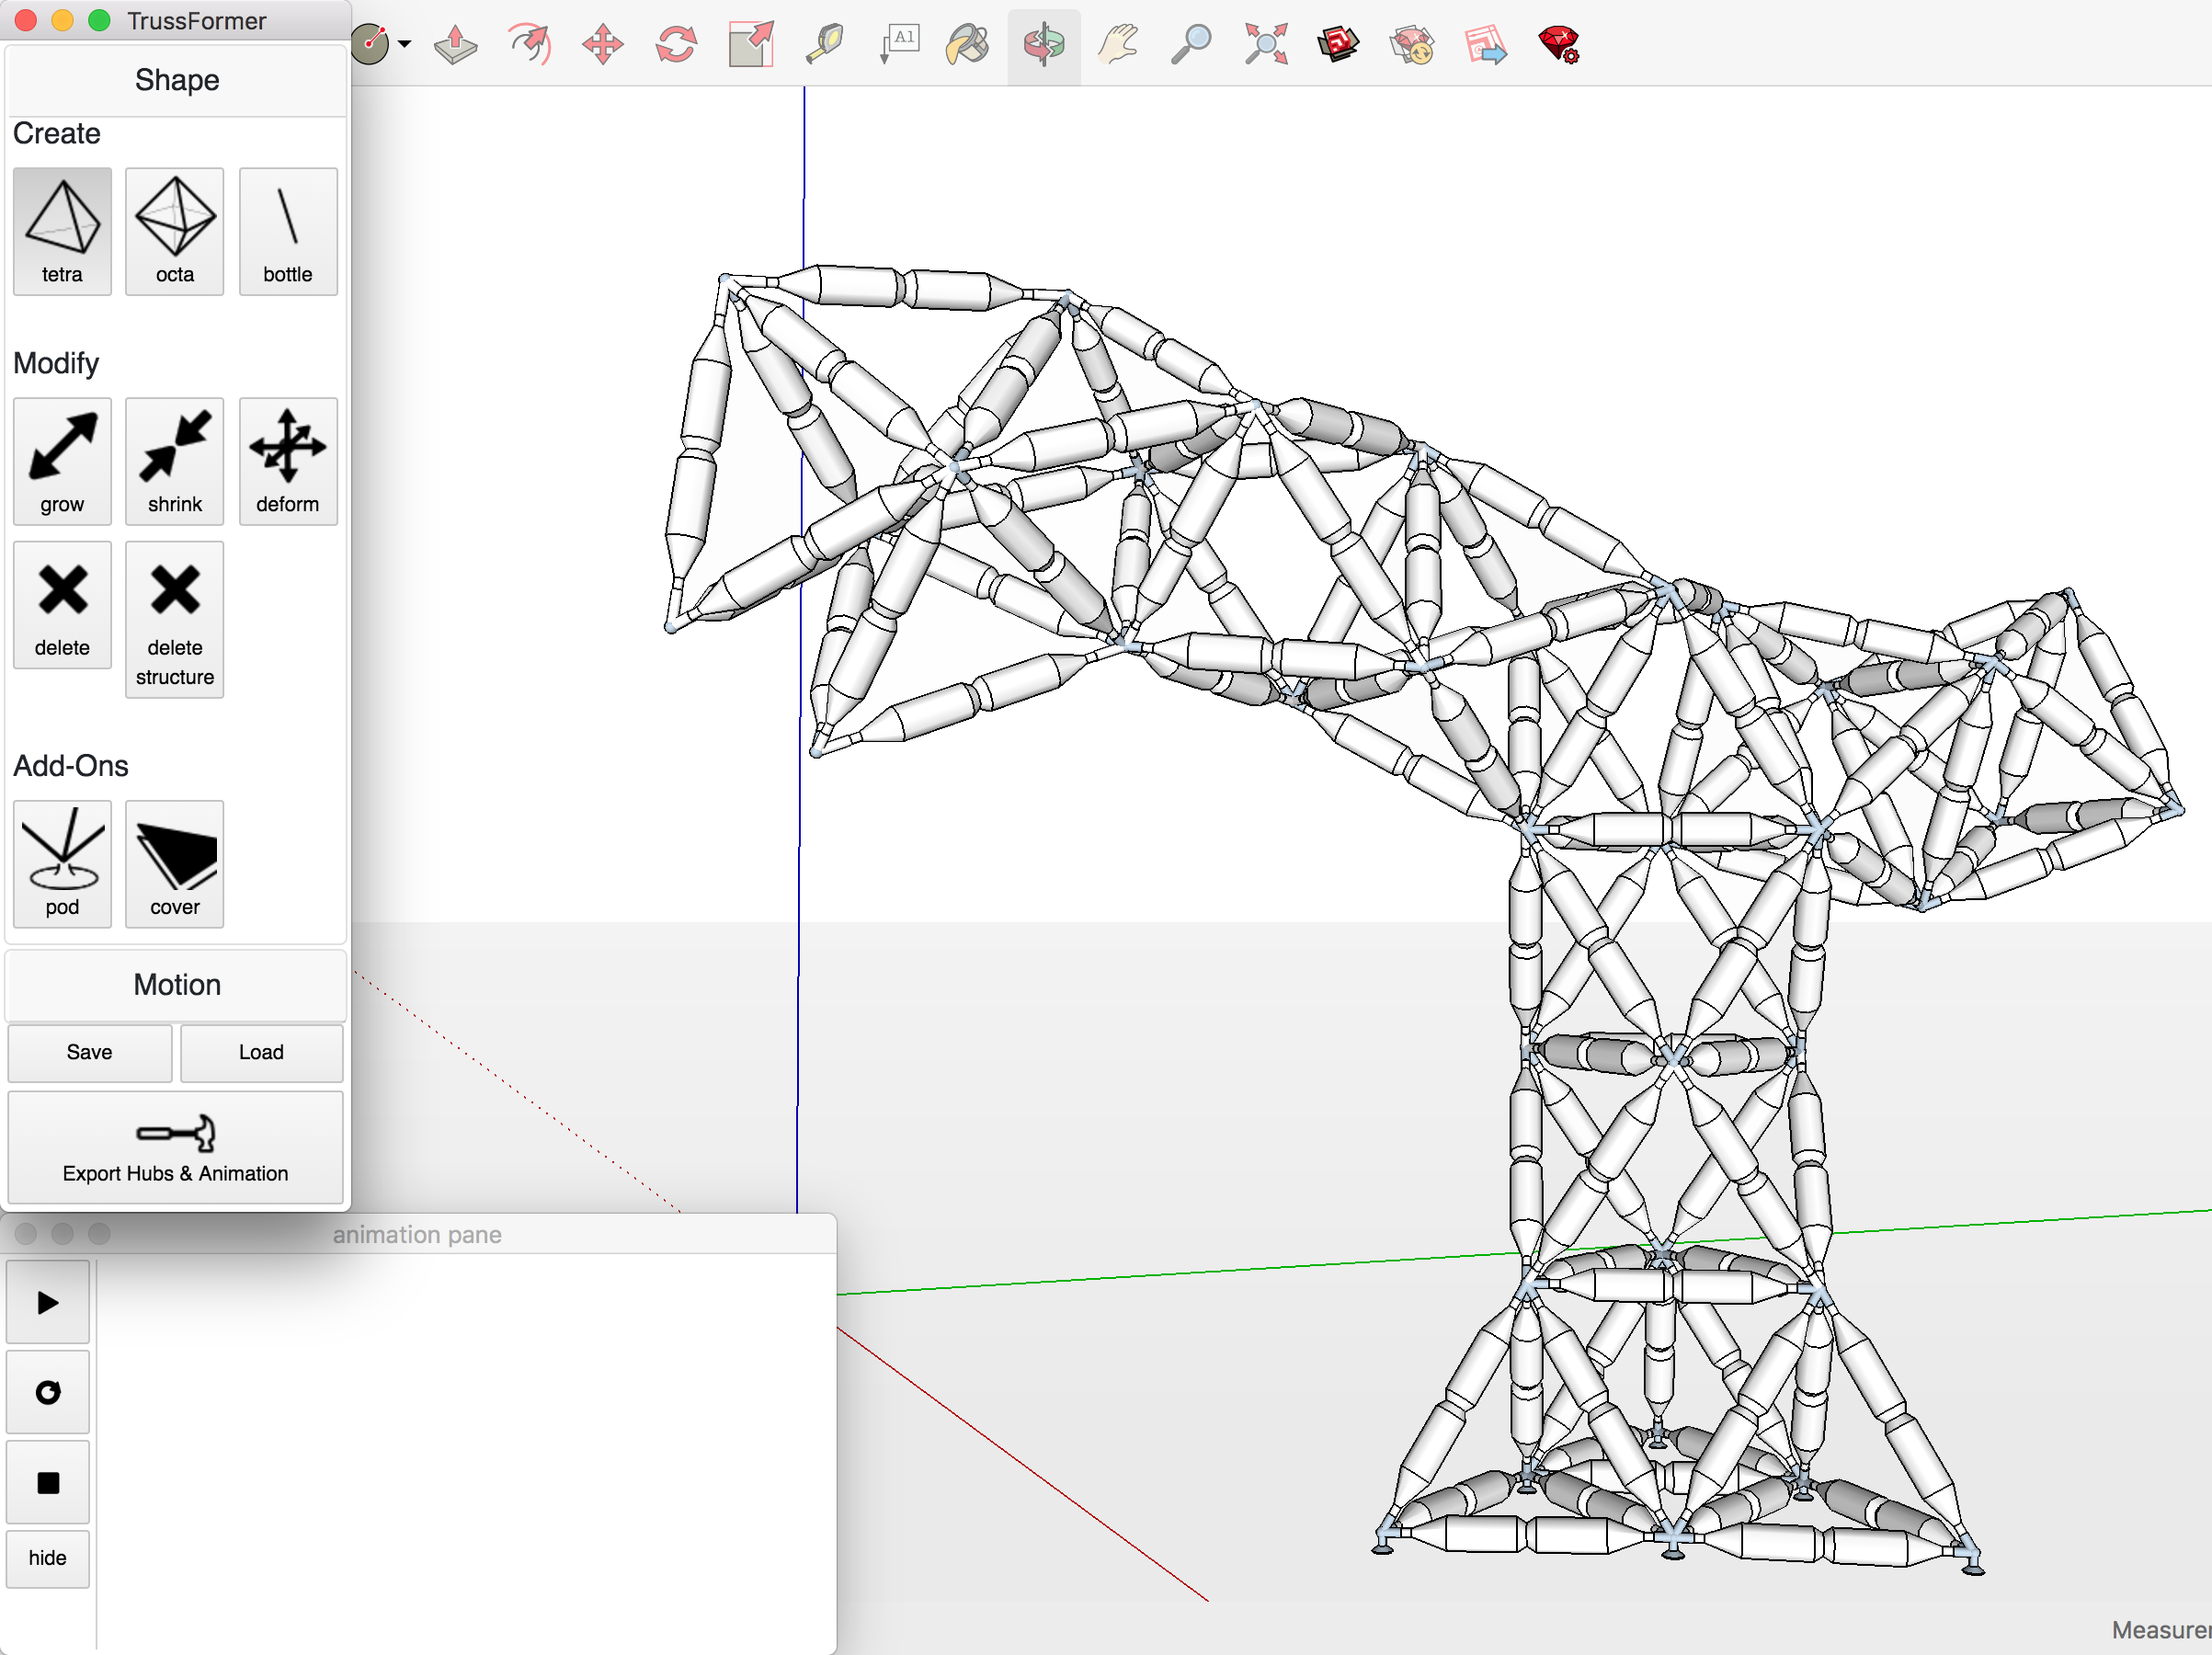
\includegraphics[width=\textwidth]{Walkthrough/dino.png}
    \centering
    \caption{The T-Rex built in TrussFab}
    \label{fig:sketchup_objects}
\end{figure}\improvement{Don't show animation pane...}
This chapter will present the functionalities of the system by showing the process of creating the T-Rex shown in figure \textit{TODO: Add image}. This will include all steps from creating the static structure, over introducing animation up to fabricating the final object.

\section{Designing Static Structures}
Users can use predefined and structurally stable primitives to create their objects. These primitives are tetrahedra and octahedra. The structure can be formed as desired by using the grow and shrink tool. These tools elongate or shorten edges, deforming the structure dynamically in such a way that the form stays in tact as much as possible. The deform tool does a similar job, but rather than working on edges, this tool can move nodes.\\
The created Objects can also be saved to a JSON file. This way the user can either save his work for working on it later or create new primitives that can be attached to another object.
\begin{figure}
  \centering
  \begin{minipage}{.5\textwidth}
    \centering
    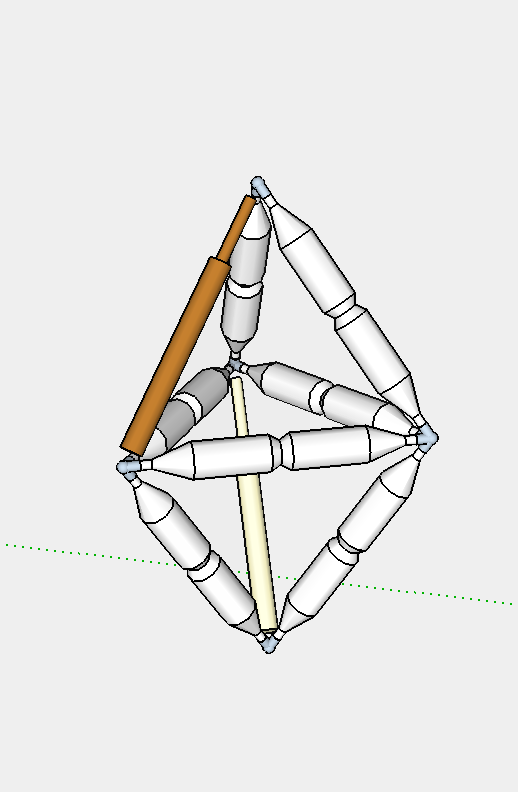
\includegraphics[width=.9\linewidth]{Walkthrough/leg_asset.png}
    \captionof{figure}{An exported leg asset...}
    \label{fig:leg_asset}
  \end{minipage}%
  \begin{minipage}{.5\textwidth}
    \centering
    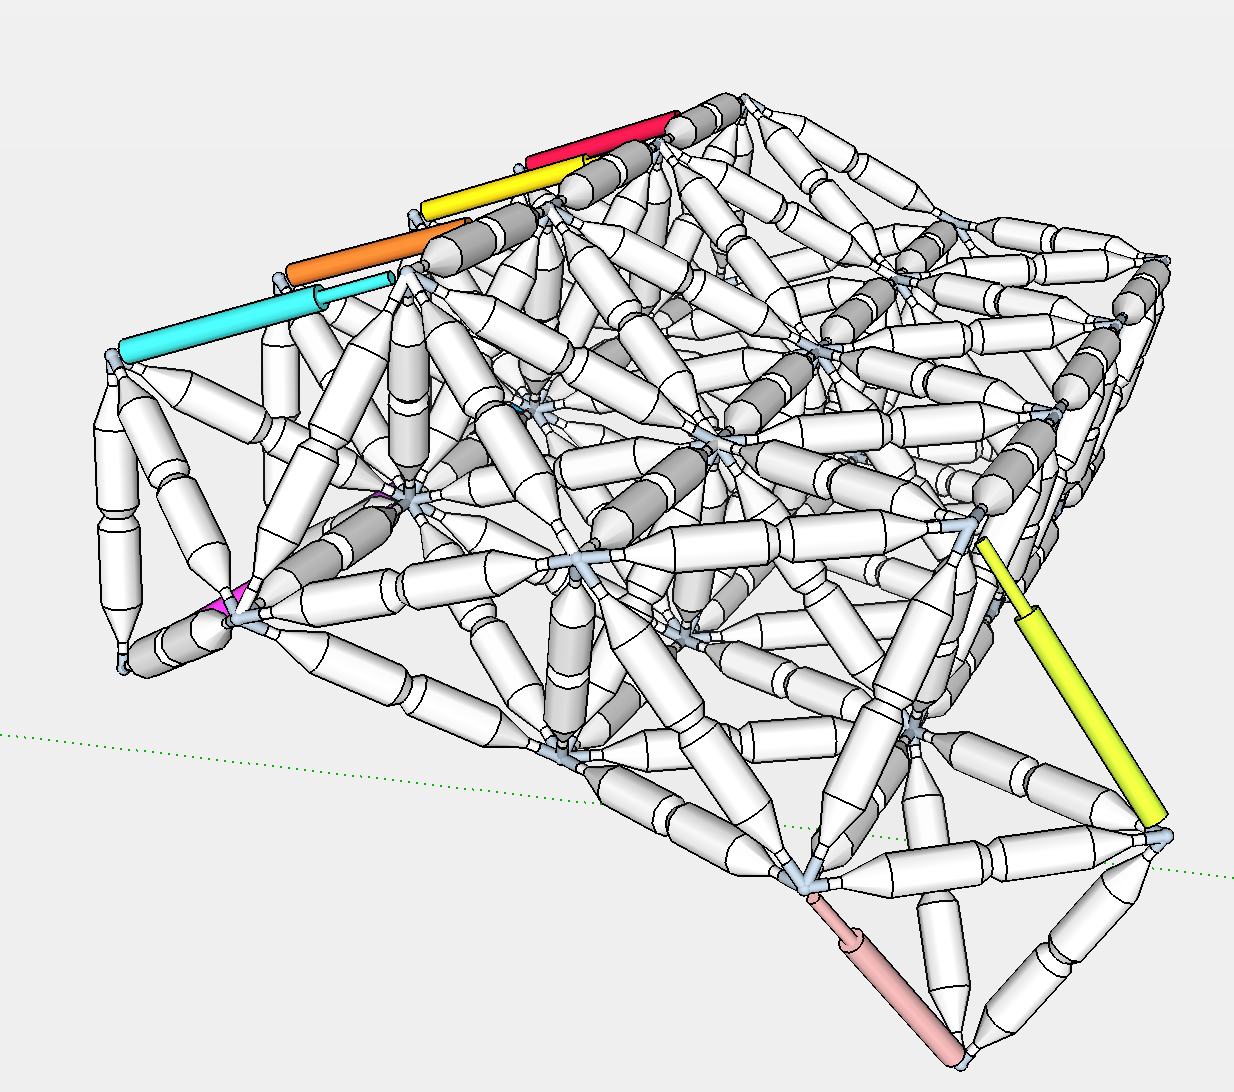
\includegraphics[width=.9\linewidth]{Walkthrough/spider_using_leg_asset.png}
    \captionof{figure}{... which can be used to quickly build the spider}
    \label{fig:spider_in_progress}
  \end{minipage}
\end{figure}

\section{Adding Movement to the Structures}
Movement is added to the structure by placing special physics links. These links act like linear actuators - struts that can extend and retract in a straight line. There are multiple methods for placing these actuators, ranging from a fully-automated way to manual placement.
\begin{figure}
  \centering
  \begin{minipage}{.5\textwidth}
    \centering
    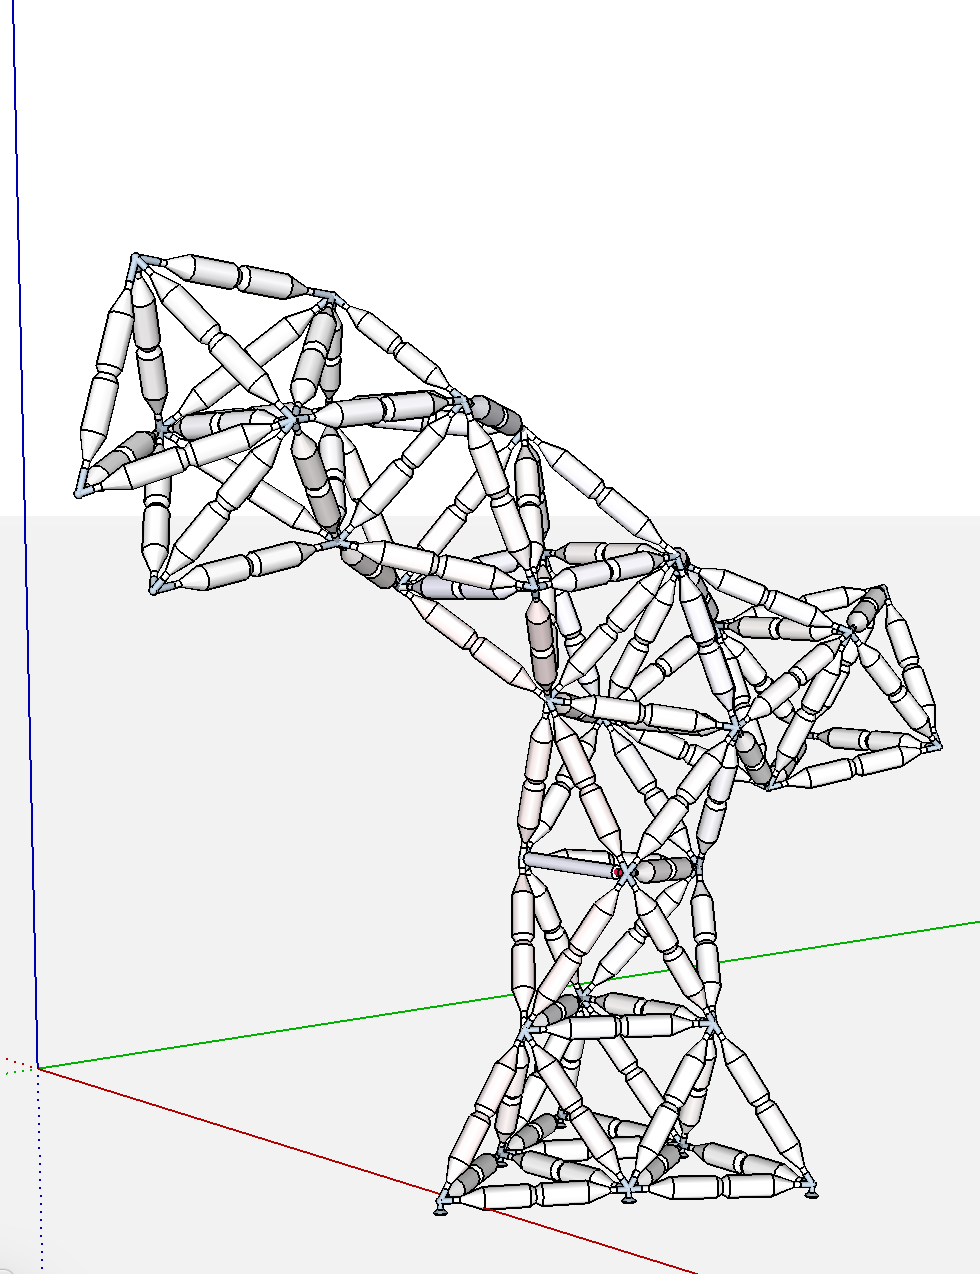
\includegraphics[width=.9\linewidth]{Walkthrough/crane_up.png}
    \captionof{figure}{An exported leg asset...}
    \label{fig:leg_asset}
  \end{minipage}%
  \begin{minipage}{.5\textwidth}
    \centering
    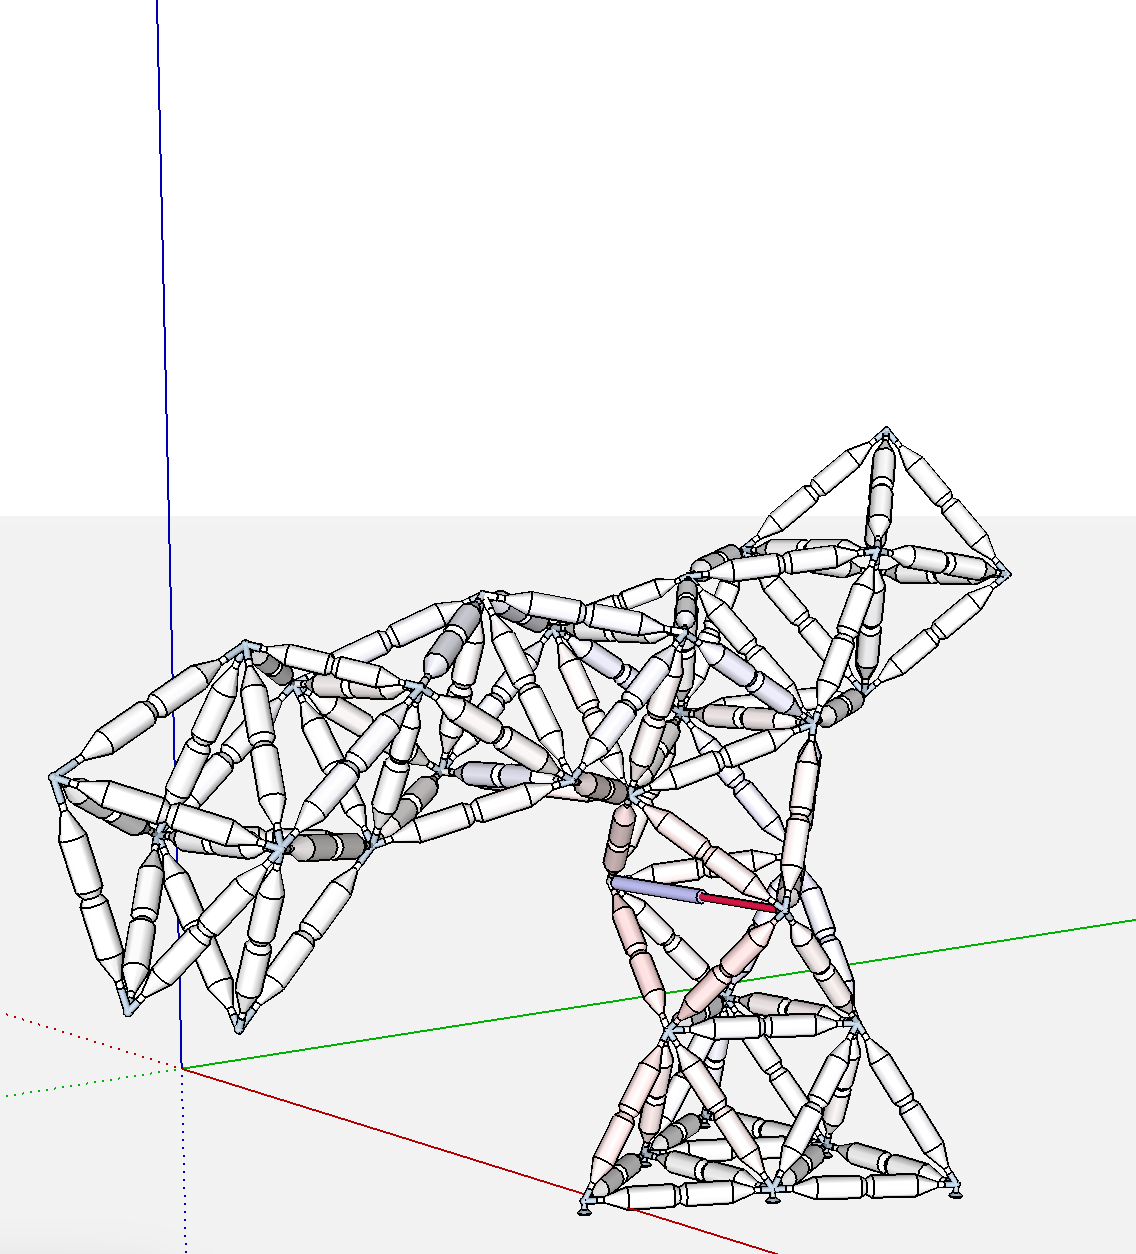
\includegraphics[width=.9\linewidth]{Walkthrough/crane_down.png}
    \captionof{figure}{... which can be used to quickly build the spider}
    \label{fig:spider_in_progress}
  \end{minipage}
\end{figure}
The automated way works by demonstrating a desired movement. The user selects the \textit{Demonstrate Movement Tool}, clicks a node that should experience a certain movement and drags a line to the desired end position. TrussFab will then search for an actuator that brings the node closest to the desired position and turns the resulting edge into an actuator. The tool runs through all edges of the structure, replacing one after another with an actuator and simulates the resulting movement in the background. The actuator that solves the problem the best will be created.\\
Another way to add movement is to use predefined dynamic assets. It can be difficult for a user to fully grasp how an actuator will move the whole object. That's why we encapsulated often-used atomic sub-assemblies into quick-access tools. These assets connect to the rest of the structure through a dedicated triangle surface. Because the motion is localized in this asset, the result in the bigger structure is easier understandable.\\
The manual actuator placement requires the most knowledge about the resulting motion. It is, however, the most flexible way to create movement. The user can choose the actuator tool to turn every edge into or connect two nodes with an actuator. This can be done by clicking on the desired edge or the nodes. Transforming an existing edge is usually the desired use case, as the introduction of more edges (by connecting two previously unconnected nodes) tends to make the truss more stable and can prevent motion altogether. Turning an edge into an actuator essentially removes this edge and adds a degree of freedom.
\subsection{Force Analysis}
If the structure fulfills the desired motion, the user will want to check if the forces created during executing it will not exceed the breaking force of the object. A lot of factors play a role in the formation of the forces. These range from weight forces over lever forces to inertial forces. TrussFab aids the user to detect weak points and force peaks during a motion in different ways.\\
TrussFab's tools provide the possibility to constantly monitor the forces that occur during interactive movement of the structure. In simulation mode, all edges will be colored red or blue in increasing intensity the higher the force on them is. Red indicates compression force, while blue means tension force. A completely white color indicates a force of 0 N. These tension forces are automatically calculated by the built-in physics engine.\\
On top of the coloring of edges, the user can also use a sensor tool. This tool can be used on a single edge and observes this one more closely. The force data on an edge with a sensor will be recorded and visualized over time in a chart. This tool also works on nodes. Rather than recording the force, if the sensor tool is used on nodes, speed and acceleration data will be visualized. The result can be seen in figure \ref{fig:sensor}.\\
\begin{figure}[h!]
    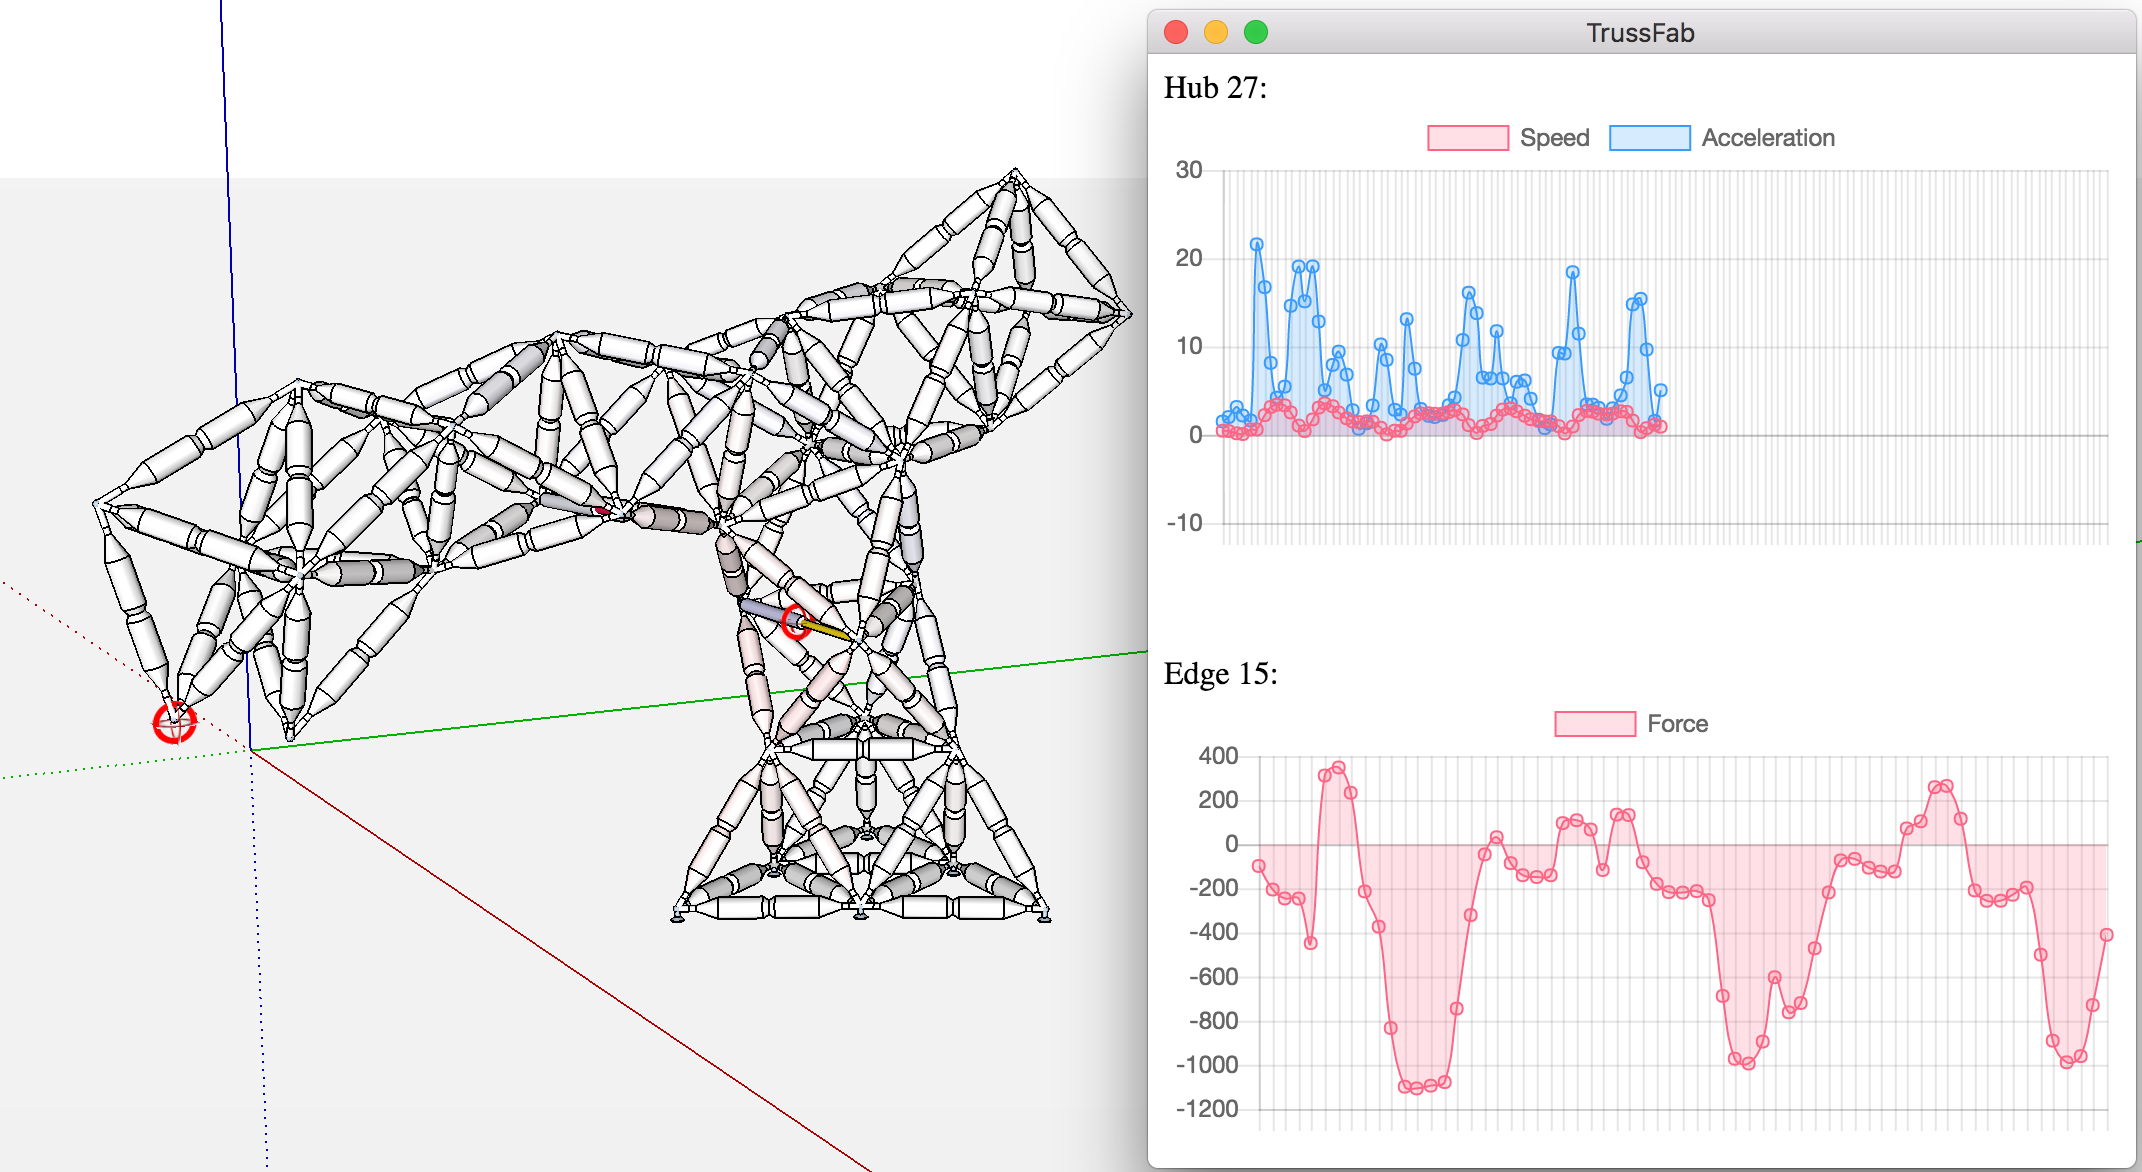
\includegraphics[width=\textwidth]{Walkthrough/sensor.png}
    \centering
    \caption{A sensor measures the force on the central actuator, and speed and acceleration on a node at the ``nose'' of the dino}
    \label{fig:sensor}
\end{figure}
- check acceleration and speed on nodes\\
- add loads to object\\
- check tension while moving\\
- automatically fix movement when object is exceeding force\\
\section{Controlling the Structure}
- closed-loop control -> more sophisticated and complex movements possible\\
\subsection{PID Control}
- short intro: how does PID work?\\
- how do we use it?\\
- i.e. position control of actuators\\
- forward reference to section 4 (setup of length measurement)\\
\section{Building the Final Object}
After the object was sufficiently tested in the editor, it is time to print the connectors and assemble the final object.
\subsection{OpenSCAD}
At first, our abstract description of the object has to be converted into a physical representation. In order to achieve this, we used a modeling language called \textit{OpenSCAD}. The \textit{Export Hubs and Hinges} button will automatically morph the structure into a statically sound object, i.e. it will elongate and shorten edges so, that the ideal amount of movement is possible. \improvement{This needs to be more detailed for sure!!}\\
The resulting arrangement of nodes and edges will be transferred to OpenSCAD. Using templates, we can create parameterized representations of hubs and hinges, which, when assembled, will exactly represent the object in the editor. This will be explained in more detail in \ref{sec:openscad_impl}.
\subsection{Printing the Parts}
Each OpenSCAD file represents a single part in the structure. These files can easily be converted to \textit{.stl} files \improvement{put conversion script in here somehow}, which are typically used for 3D printing. These files have to be imported into any 3D printing software, arranged efficiently and send to a 3D printer. \unsure{add some time reference here?}
\subsection{Assembling the Structure}
The resulting hubs and hinges contain an ID system for easy assembly. Each part of a node has the node ID printed on. That way it is easy to find out which hinge-parts belong together. Additionally, each ``extended'' edge-line (elongation) \info{Verlängerung einer Edge, also quasi die Elongation. FIND A BETTER NAME!} contains the id of the connected edge. A compound elongation, which is the usual case for a hinge, is therefore assembled by finding two parts with the same node and edge ID. For static hubs, this concept is similar, but of course these do not have to be assembled.\\
Two connectors with different node IDs but the same edge IDs will be connected by a link.
